\documentclass[tikz]{standalone}
\usepackage{tikz}
\usepackage{alphalph}
\usetikzlibrary{positioning, graphs}
\usetikzlibrary{graphs.standard}
\begin{document}
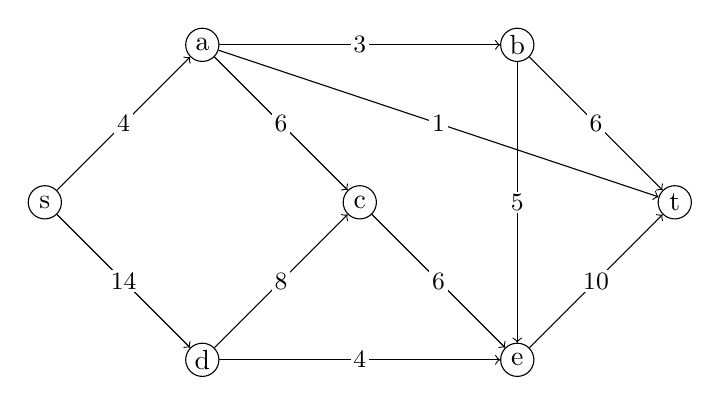
\begin{tikzpicture}
\begin{scope}
		[vertex/.style={draw,circle,inner sep = 0em, minimum size = 1.2em},
		 edgelabel/.style = {fill = white, inner sep = 0.1em, font=\small}]
		\node[vertex] (a) at (0,0) {a};
		\node[vertex] (b) at (4,0) {b};
		\node[vertex] (s) at (-2,-2) {s};
		\node[vertex] (c) at (2,-2) {c};
		\node[vertex] (t) at (6,-2) {t};
		\node[vertex] (d) at (0,-4) {d};
		\node[vertex] (e) at (4,-4) {e};
		
		\draw[->] (s) to node[edgelabel] {4} (a);
		\draw[->] (s) to node[edgelabel] {14} (d);
		\draw[->] (a) to node[edgelabel] {3} (b);
		\draw[->] (a) to node[edgelabel] {6} (c);
		\draw[->] (a) to node[edgelabel] {1} (t);
		\draw[->] (b) to node[edgelabel] {5} (e);
		\draw[->] (b) to node[edgelabel] {6} (t);
		\draw[->] (c) to node[edgelabel] {6} (e);
		\draw[->] (d) to node[edgelabel] {8} (c);
		\draw[->] (d) to node[edgelabel] {4} (e);
		\draw[->] (e) to node[edgelabel] {10} (t);
		
\end{scope}
\end{tikzpicture}
\end{document}